\begin{center}
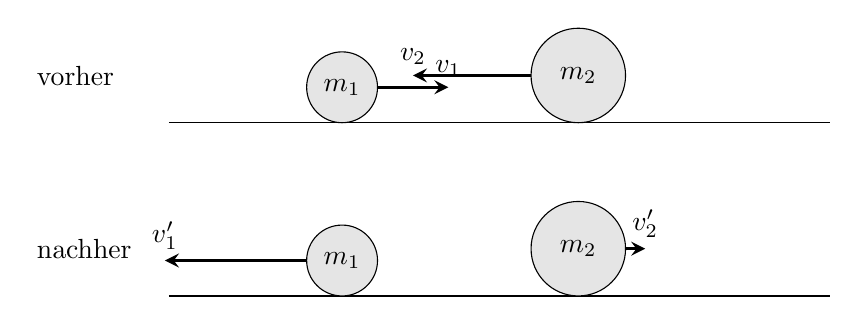
\begin{tikzpicture}[>=stealth]
 \node[anchor=west] at (0,0.6) {vorher};
 \draw (1.8,0) -- (10.2,0);
 \draw[fill=gray!20] (4,0.45) circle (0.45);
 \node at (4,0.45) {$m_1$};
 \draw[->, very thick] (4.45,0.45) -- (5.35,0.45) node[above] {$v_1$};
 \draw[fill=gray!20] (7,0.6) circle (0.6);
 \node at (7,0.6) {$m_2$};
 \draw[->, very thick] (6.4,0.6) -- (4.9,0.6) node[above] {$v_2$};
 \node[anchor=west] at (0,-1.6) {nachher};
 \draw (1.8,-2.2) -- (10.2,-2.2);
 \draw[fill=gray!20] (4,-1.75) circle (0.45);
 \node at (4,-1.75) {$m_1$};
 \draw[->, very thick] (3.55,-1.75) -- (1.75,-1.75) node[above] {$v_1'$};
 \draw[fill=gray!20] (7,-1.6) circle (0.6);
 \node at (7,-1.6) {$m_2$};
 \draw[->, very thick] (7.6,-1.6) -- (7.85,-1.6) node[above] {$v_2'$};
\end{tikzpicture}
\end{center}

Die Bewegungsrichtung der ersten Kugel vor dem Stoss ist positiv. Mit den Beträgen $v_1 = \vEaO$, $v_2 = \vZaO$, $v_1' = \vEeO$ und $v_2' = \vZeO$ lautet die Impulserhaltung
\begin{align}
 m_1\,v_1 - m_2\,v_2 &= -m_1\,v_1' + m_2\,v_2' \\
 m_1\left(v_1+v_1'\right) &= m_2\left(v_2+v_2'\right)
\end{align}
Das Massenverhältnis ist also
\begin{align}
 \frac{m_1}{m_2} &= \rMF \\
   &= \frac{\vZa+\vZe}{\vEa+\vEe} \\
   &= \rM \approx \result{\rMP{0}{2}}
\end{align}
Die zweite Kugel ist doppelt so schwer wie die erste, $m_1 : m_2 = 1 : 2$.
